\section{Flavour changing neutral currents}
\label{sec:fcncs}

Flavour-changing neutral currents (FCNCs) are quark transitions which change the generation of the quark without any total change in electric charge.
FCNC processes are forbidden at tree level in the SM as shown above but can occur in 
loop processes where the mediating \Wpm boson is entirely virtual such as a \bquark\to\squark transition.
The \bquark\to\squark loop can radiate a photon (\btosgam) and or dilepton (\bsll) with 
either a penguin or box internal structure.
Examples of different \bsll transitions in the SM are shown in Fig.~\ref{fig:bssm}.
\begin{figure}[tbp]
\centering
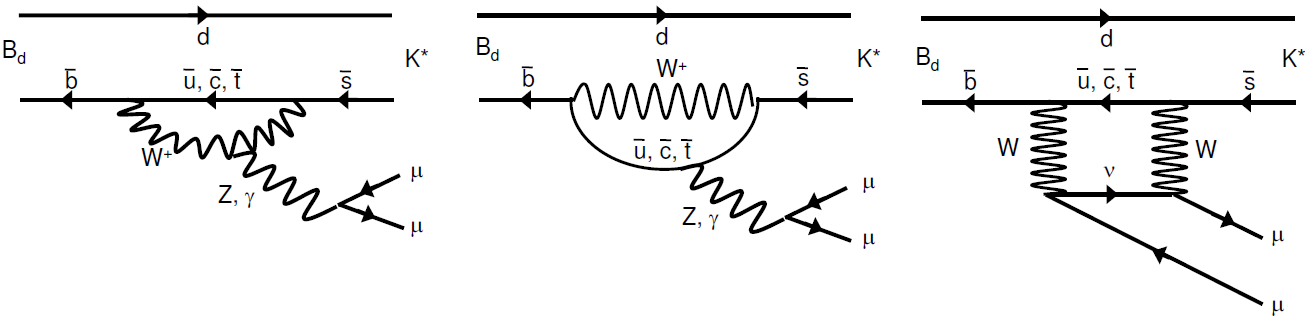
\includegraphics[width=0.66\columnwidth]{chapter2/figs/Feyn.png}
\caption[Feynman diagrams for a b to s transition]
{Three different Feynman diagrams showing the SM process that allow a \bsll transition,
 two penguin diagrams and a \W box diagram. ~\label{fig:bssm}}
\end{figure}
Processes which contain a \bquark\to\squark transition are popular FCNC decays for tests of contributions from new physics~\cite{Melikhov:1998cd}.
Measurements of FCNCs are model-independent tests of any new physics model that contribute to change the overall properties of the decay.

The formalism of \bquark-hadron decays can be expressed in terms of an effective theory, which separates different contributions to the decay 
by a particular mass scale. 
The effective theory of \B decays, Heavy Quark Effective Theory~\cite{Mannel:2004ce,Manohar:2000dt} ,
separates out particles with masses much greater than that of a \bquark quark, 
such as the electroweak gauge bosons, the Higgs, the \tquark quark and any new massive particles.
The operator product expansion separates these high and low energy contributions into a set of coefficients and operators~\cite{Wilson:1972ee},
\begin{align}
\bra{f}\mathcal{H}\ket{i} &=  \sum_k \C{k}(\mu) \bra{f}\Ope{k} (\mu)\ket{i}  \, ,
\end{align}
where the Wilson coefficients ($C$) and the operators ($O$) are normalised to a mass scale ($\mu$).

The operators encode the low energy contributions from the quarks in the decay and the Wilson coefficients encode
 the contributions from higher mass particles above the mass scale $\mu$.
For this reason the Wilson coefficients are said to encode the `short' distance physics whilst the 
operators encode the `long' distance physics.
The short distance physics covers everything above the mass scale of the effective Hamiltonian, 
such weak interactions and any contribution from physics beyond the SM.
The long distance physics covers everything below the mass scale of the Hamiltonian, 
\ie~the \Kstar physics and the interactions with the light spectator quark.
The benefit of this formalism is that the Wilson coefficients can include arbitrary contributions from new physical models and 
provide a model-independent formalism through which to measure these contributions.

The effective Hamiltonian for the \bsll transition~\cite{AltmannshoferBall} is
\begin{align}
H = \frac{4G_F}{\sqrt{2}} V_{tb}^{*} V_{ts} \sum_{i=1}^{10} C_i(\mu) O_i(\mu) \, .
\end{align}
The electroweak penguin operators are 
\begin{subequations}\begin{align}
\Ope{7}  &= \frac{e}{g^2}  m_b\left(\bar{\squark}\sigma_{\mu\nu}\frac{1}{2}(1\pm\gamma^5)\bquark\right) F^{\mu\nu}   \, , \\
\Ope{8}  &= \frac{1}{g} m_b\left(\bar{\squark}\sigma_{\mu\nu}T^a\frac{1}{2}(1\pm\gamma^5)\bquark\right) G^{a,\mu\nu}   \, , \\
\Ope{9}  &= \frac{e^2}{g^2} m_b\left(\bar{\squark}\gamma_\mu\frac{1}{2}(1\mp\gamma^5)\bquark\right) (\bar{\ell} \gamma^\mu \ell ) \, , \\
\Ope{10}  &= \frac{e^2}{g^2} m_b\left(\bar{\squark}\gamma_\mu\frac{1}{2}(1\mp\gamma^5)\bquark\right) (\bar{\ell} \gamma^\mu \gamma^5 \ell ) \, ,
\end{align}\end{subequations}
where $g$ is the strong coupling constant and $m_b$ is the \bquark mass dependent on the chosen renormalisation scheme.
The operator \Ope7  describes the electroweak penguin decay with a photon propagator, \Ope8 describes the diagram with a gluon propagator 
and the operators \Ope9 and \Ope10 describe the diagrams with electroweak bosons, either \Wpm or \Z.
The respective Wilson coefficients for these quark transitions are \C7 , \C8 , \C9 and \C{10} ~\cite{Bobeth:1999mk}.
The Wilson coefficients at the \bquark mass are evolved down from the weak mass scale, giving effective Wilson coefficients which also
include contributions from the four-quark and gluonic operators \C{1\to6},
\begin{align}
\Ceff7 &= \frac{4\pi}{\alpha_S} \C7 - \frac{1}{3} \C3 - \frac{4}{9} \C4 - \frac{20}{3} \C5 - \frac{80}{9} \C6 , \\
\Ceff8 &= \frac{4\pi}{\alpha_S} \C8 + \C3 - \frac{1}{6} \C4 + 20 \C5 - \frac{10}{3} \C6 , \\
\Ceff9 &= \frac{4\pi}{\alpha_S} \C9 + Y(\qsq) \\
\Ceff10 &= \frac{4\pi}{\alpha_S}\C{10} \\
\Ceff_{7,8,9,10} &= \frac{4\pi}{\alpha_S}\Cpeff{7,8,9,10} \, .
\end{align}
where Y(\qsq), along with more detail about the effective coefficients can be found in Ref~\cite{AltmannshoferBall}.
Contributions from physics beyond the SM can also be parameterised in terms of the Wilson coefficients.
Right handed currents for each operator can be introduced as primed counterparts to the SM Wilson coefficients (\Cp{7}, \Cp{8}, \Cp{9} and \Cp{10} ) and 
 contributions from new scalars and pseudoscalar particles can be incorporated in the form of additional Wilson coefficients \C{S} and \C{P} .

Constraints on the Wilson coefficients can be obtained from measurements of different FCNCs~\cite{Altmannshofer:2012az}.
Measurements of \btosgam transitions are proportional to the magnitude of \C{7} and measurements of 
\bsll transitions in the form of \Bsmm are proportional the value of \C10 and could incorporate contributions from \C{S} and \C{P} .
The \bsll electroweak penguin decay is mainly parameterised by \C{7}, \C9 and \C{10} , allowing 
 measurements of the \bsll decays to constrain a wide range of models of physics beyond the SM.

%Theoretical predictions for each of the Wilson coefficients come from several methods depending on the energy given to 
%the \ellell and \kpi pair.
%For the energy region where the \Kstarz meson carries a large proportion of the available energy,
% the `large recoil' region, a technique called QCD factorisation can be used~\cite{Beneke:2000wa}.
% \emph{ QCD factorisation does something I still don't understand }
%There are two other regions, the dimuon range close to the charmonium (\jpsi and \psitwos) resonances 
% and the limit of soft \Kstarz and high momentum dimuon where two different approaches must be taken, as described in 
% Refs~\cite{Khodjamirian:2010vf} and~\cite{Bobeth:2011nj} respectively.

